\documentclass[tikz,border=7pt]{standalone}
\usepackage{amsmath}
\usepackage{amssymb}
\usetikzlibrary{calc,arrows.meta,decorations.pathreplacing}

% Muted palette only. White is used only for the page/background.
\definecolor{mistyblue}{HTML}{A3BFD9}
\definecolor{slateblue}{HTML}{7A90B2}
\definecolor{sagegreen}{HTML}{A3BFA3}
\definecolor{dustyteal}{HTML}{6E8B8B}
\definecolor{softgray}{HTML}{D8D8D8}
\definecolor{deepmutedblue}{HTML}{4A5A6A}

\colorlet{ink}{deepmutedblue}
\colorlet{line}{slateblue}
\colorlet{gridline}{softgray}

\colorlet{blueA}{slateblue}
\colorlet{blueFill}{mistyblue}
\colorlet{blueDash}{dustyteal}

\colorlet{amberA}{dustyteal}
\colorlet{amberFill}{sagegreen}
\colorlet{amberDash}{slateblue}

\colorlet{greenA}{deepmutedblue}
\colorlet{greenFill}{sagegreen}
\colorlet{greenDash}{dustyteal}

\begin{document}
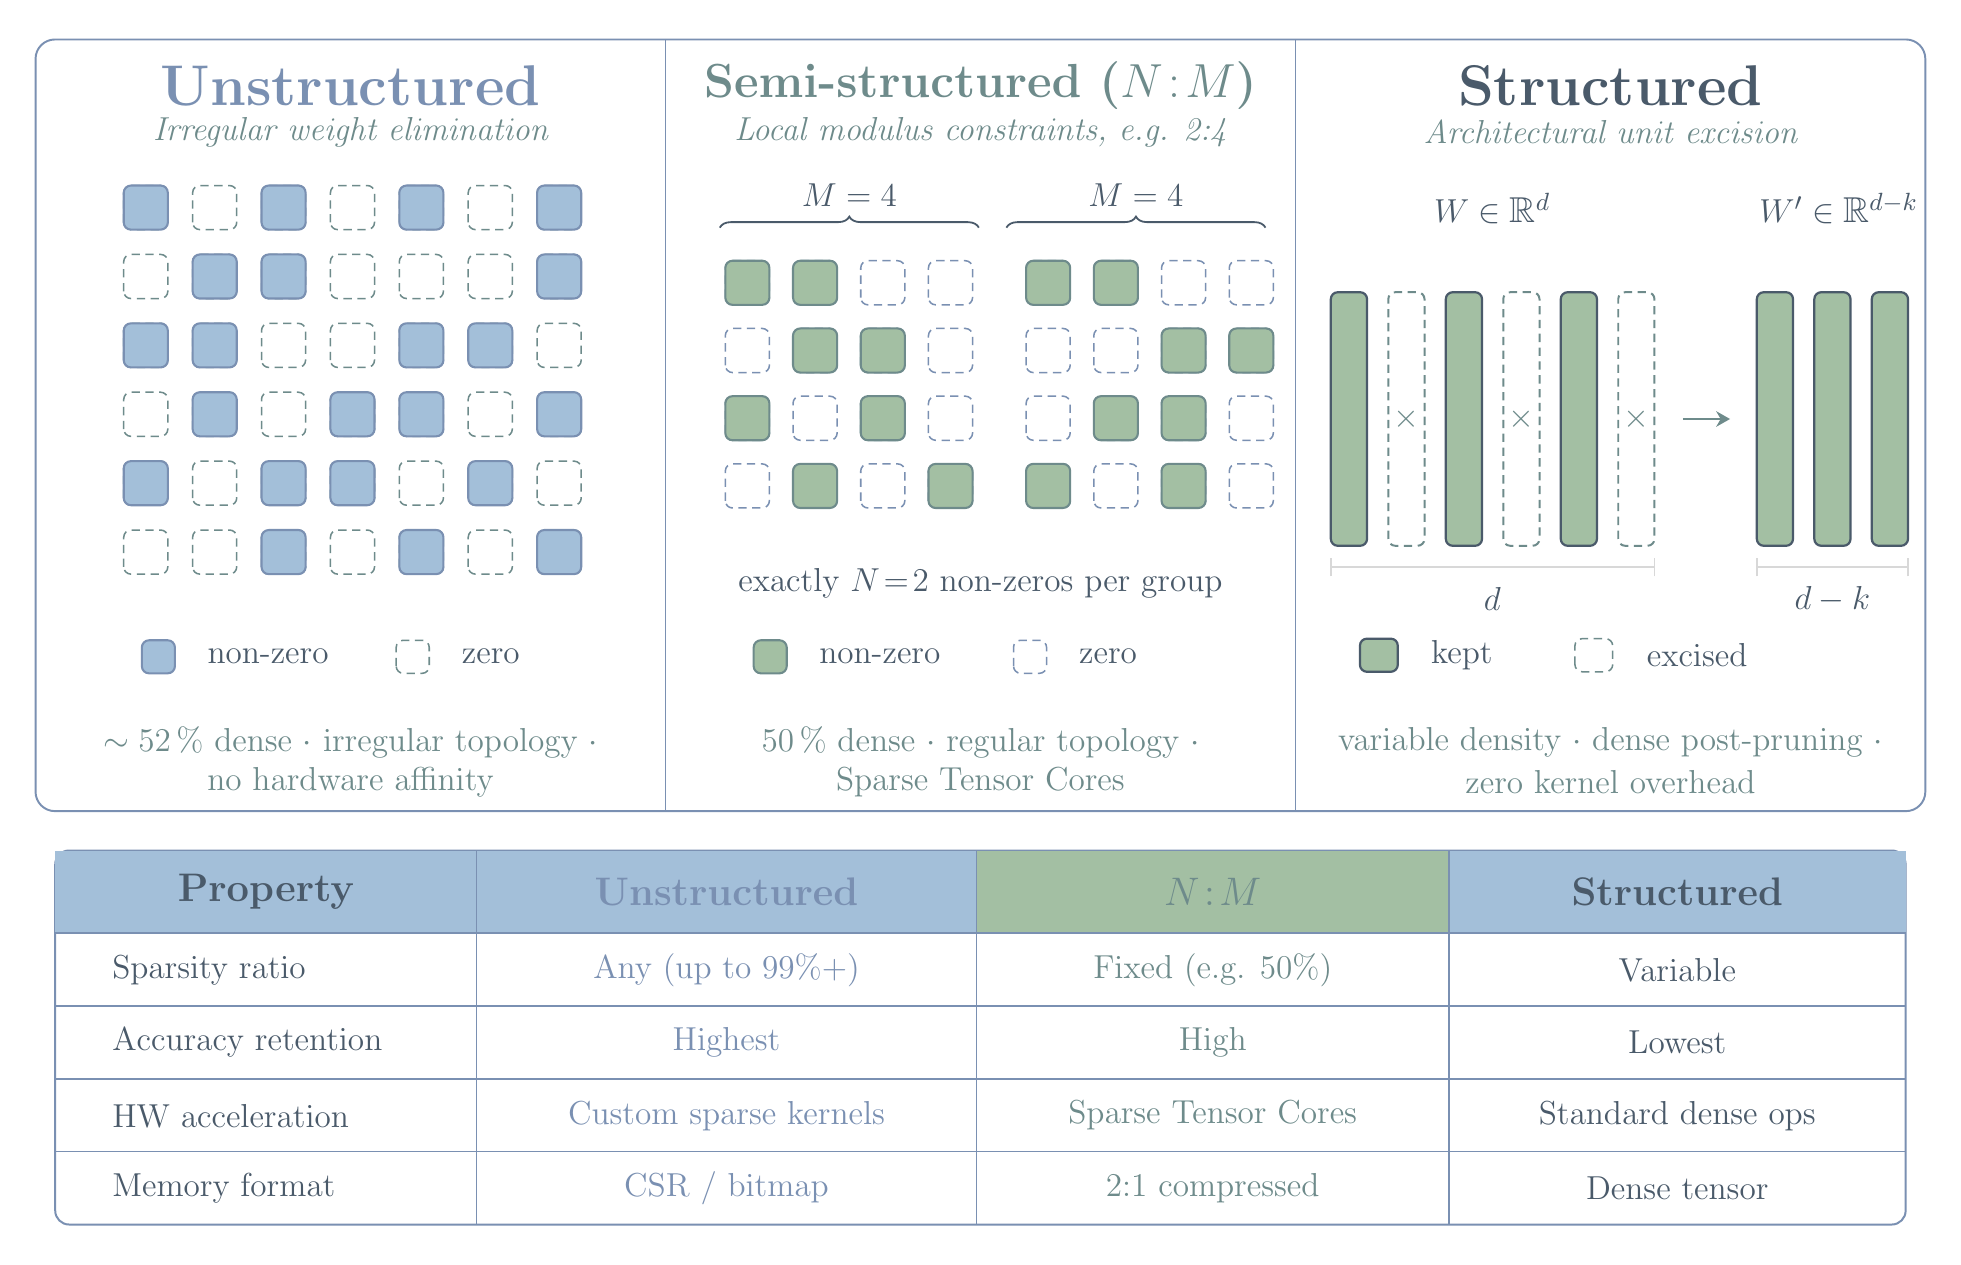
\begin{tikzpicture}[
  x=1cm,y=1cm,
  >=Stealth,
  every node/.style={font=\rmfamily, text=ink},
  title/.style={font=\rmfamily\bfseries\fontsize{21}{24}\selectfont},
  subtitle/.style={font=\rmfamily\itshape\fontsize{12}{15}\selectfont, text=dustyteal},
  small/.style={font=\rmfamily\fontsize{11}{13}\selectfont},
  body/.style={font=\rmfamily\fontsize{13}{15}\selectfont},
  tabhead/.style={font=\rmfamily\bfseries\fontsize{14}{16}\selectfont},
  cellText/.style={font=\rmfamily\fontsize{11.5}{14}\selectfont},
  note/.style={font=\rmfamily\fontsize{11.8}{14}\selectfont, text=dustyteal},
  zeroCell/.style={rounded corners=2.6pt, line width=0.55pt, densely dashed},
  fullCell/.style={rounded corners=2.6pt, line width=0.75pt},
  barFull/.style={rounded corners=2.5pt, line width=0.8pt},
  barZero/.style={rounded corners=2.5pt, line width=0.72pt, densely dashed},
  arr/.style={-{Stealth[length=5pt,width=5.6pt]}, line width=0.95pt, draw=dustyteal},
  brace/.style={decorate, decoration={brace, amplitude=4pt}, line width=0.65pt, draw=ink}
]

% ---------------------------------------------------------------------------
% Global layout constants
% Width = 24.0 cm.  Three top panels of 8.0 cm each.
% Top panel: y = 5.45 .. 15.25. Bottom table: y = 0.20 .. 4.95.
% ---------------------------------------------------------------------------
\fill[white] (-0.10,0.05) rectangle (24.10,15.40);

% =============================== TOP PANELS ===============================
\draw[line, rounded corners=7pt, line width=0.7pt] (0,5.45) rectangle (24,15.25);
\draw[line, line width=0.55pt] (8,5.45) -- (8,15.25);
\draw[line, line width=0.55pt] (16,5.45) -- (16,15.25);

% ----------------------------- Unstructured -------------------------------
\node[title, text=blueA] at (4,14.67) {Unstructured};
\node[subtitle] at (4,14.07) {Irregular weight elimination};

% Unstructured grid: 7 columns x 6 rows, 0.56 cell, 0.315 gap.
\def\ucx{1.12}
\def\ucy{8.46}
\def\ucs{0.56}
\def\ucg{0.315}
\foreach \r in {1,...,6}{
  \foreach \c in {1,...,7}{
    \pgfmathsetmacro{\xx}{\ucx + (\c-1)*(\ucs+\ucg)}
    \pgfmathsetmacro{\yy}{\ucy + (6-\r)*(\ucs+\ucg)}
    \draw[zeroCell, draw=blueDash] (\xx,\yy) rectangle ++(\ucs,\ucs);
  }
}
\foreach \r/\c in {
  1/1,1/3,1/5,1/7,
  2/2,2/3,2/7,
  3/1,3/2,3/5,3/6,
  4/2,4/4,4/5,4/7,
  5/1,5/3,5/4,5/6,
  6/3,6/5,6/7
}{
  \pgfmathsetmacro{\xx}{\ucx + (\c-1)*(\ucs+\ucg)}
  \pgfmathsetmacro{\yy}{\ucy + (6-\r)*(\ucs+\ucg)}
  \draw[fullCell, draw=blueA, fill=blueFill] (\xx,\yy) rectangle ++(\ucs,\ucs);
}

% Legend - unstructured
\draw[fullCell, draw=blueA, fill=blueFill] (1.35,7.20) rectangle ++(0.42,0.42);
\node[body, anchor=west] at (2.06,7.41) {non-zero};
\draw[zeroCell, draw=blueDash] (4.58,7.20) rectangle ++(0.42,0.42);
\node[body, anchor=west] at (5.29,7.41) {zero};

\node[note, align=center] at (4,6.32) {$\sim 52\,\%$ dense $\cdot$ irregular topology $\cdot$};
\node[note, align=center] at (4,5.82) {no hardware affinity};

% ----------------------------- Semi-structured -----------------------------
\node[text=amberA, font=\rmfamily\bfseries\fontsize{18.5}{21}\selectfont] at (12,14.67) {Semi-structured ($N\!:\!M$)};
\node[subtitle] at (12,14.07) {Local modulus constraints, e.g. 2:4};

% Semi-structured grid: 8 columns x 4 rows. Two 4-wide groups.
\def\scx{8.76}
\def\scy{9.30}
\def\scs{0.56}
\def\scg{0.30}
\def\sgap{0.38}
\foreach \r in {1,...,4}{
  \foreach \c in {1,...,8}{
    \ifnum\c>4\def\sextra{\sgap}\else\def\sextra{0}\fi
    \pgfmathsetmacro{\xx}{\scx + (\c-1)*(\scs+\scg) + \sextra}
    \pgfmathsetmacro{\yy}{\scy + (4-\r)*(\scs+\scg)}
    \draw[zeroCell, draw=amberDash] (\xx,\yy) rectangle ++(\scs,\scs);
  }
}
\foreach \r/\c in {
  1/1,1/2,1/5,1/6,
  2/2,2/3,2/7,2/8,
  3/1,3/3,3/6,3/7,
  4/2,4/4,4/5,4/7
}{
  \ifnum\c>4\def\sextra{\sgap}\else\def\sextra{0}\fi
  \pgfmathsetmacro{\xx}{\scx + (\c-1)*(\scs+\scg) + \sextra}
  \pgfmathsetmacro{\yy}{\scy + (4-\r)*(\scs+\scg)}
  \draw[fullCell, draw=amberA, fill=amberFill] (\xx,\yy) rectangle ++(\scs,\scs);
}
% Braces over the two M groups.
\draw[brace] (8.69,12.86) -- (11.98,12.86)
  node[midway,above=4pt,font=\rmfamily\fontsize{12}{14}\selectfont] {$M=4$};
\draw[brace] (12.33,12.86) -- (15.62,12.86)
  node[midway,above=4pt,font=\rmfamily\fontsize{12}{14}\selectfont] {$M=4$};

\node[body, align=center] at (12,8.35) {exactly $N\!=\!2$ non-zeros per group};

% Legend - semi structured
\draw[fullCell, draw=amberA, fill=amberFill] (9.12,7.20) rectangle ++(0.42,0.42);
\node[body, anchor=west] at (9.83,7.41) {non-zero};
\draw[zeroCell, draw=amberDash] (12.42,7.20) rectangle ++(0.42,0.42);
\node[body, anchor=west] at (13.13,7.41) {zero};

\node[note, align=center] at (12,6.32) {$50\,\%$ dense $\cdot$ regular topology $\cdot$};
\node[note, align=center] at (12,5.82) {Sparse Tensor Cores};

% -------------------------------- Structured --------------------------------
\node[title, text=greenA] at (20,14.67) {Structured};
\node[subtitle] at (20,14.07) {Architectural unit excision};

\node[body] at (18.50,13.10) {$W\in\mathbb{R}^{d}$};
\node[body] at (22.90,13.10) {$W'\in\mathbb{R}^{d-k}$};

% Left structured block: six vertical units, alternating kept/excised.
\def\bary{8.82}
\def\barh{3.22}
\def\barw{0.46}
\def\barg{0.27}
\def\barx{16.45}
\foreach \i in {0,2,4}{
  \pgfmathsetmacro{\xx}{\barx + \i*(\barw+\barg)}
  \draw[barFull, draw=greenA, fill=greenFill] (\xx,\bary) rectangle ++(\barw,\barh);
}
\foreach \i in {1,3,5}{
  \pgfmathsetmacro{\xx}{\barx + \i*(\barw+\barg)}
  \draw[barZero, draw=greenDash] (\xx,\bary) rectangle ++(\barw,\barh);
  \node[font=\rmfamily\fontsize{13}{15}\selectfont,text=greenDash] at ({\xx+0.23},{\bary+1.61}) {$\times$};
}

% Dimension bracket under W.
\draw[gridline, line width=0.58pt] (16.45,8.55) -- (20.56,8.55);
\draw[gridline, line width=0.58pt] (16.45,8.43) -- (16.45,8.67);
\draw[gridline, line width=0.58pt] (20.56,8.43) -- (20.56,8.67);
\node[body] at (18.50,8.14) {$d$};

% Arrow and right structured block.
\draw[arr] (20.92,10.43) -- (21.52,10.43);

\def\rbarx{21.86}
\foreach \i in {0,1,2}{
  \pgfmathsetmacro{\xx}{\rbarx + \i*(\barw+\barg)}
  \draw[barFull, draw=greenA, fill=greenFill] (\xx,\bary) rectangle ++(\barw,\barh);
}
\draw[gridline, line width=0.58pt] (21.86,8.55) -- (23.78,8.55);
\draw[gridline, line width=0.58pt] (21.86,8.43) -- (21.86,8.67);
\draw[gridline, line width=0.58pt] (23.78,8.43) -- (23.78,8.67);
\node[body] at (22.82,8.14) {$d-k$};

% Legend - structured
\draw[barFull, draw=greenA, fill=greenFill] (16.82,7.22) rectangle ++(0.48,0.42);
\node[body, anchor=west] at (17.60,7.43) {kept};
\draw[zeroCell, draw=greenDash] (19.55,7.22) rectangle ++(0.48,0.42);
\node[body, anchor=west] at (20.34,7.43) {excised};

\node[note, align=center] at (20,6.32) {variable density $\cdot$ dense post-pruning $\cdot$};
\node[note, align=center] at (20,5.82) {zero kernel overhead};

% =============================== BOTTOM TABLE ===============================
\def\tx{0.25}
\def\ty{0.20}
\def\tw{23.50}
\def\th{4.75}
\draw[line, rounded corners=5pt, line width=0.72pt] (\tx,\ty) rectangle ++(\tw,\th);

% Table column positions: 5.35 | 6.35 | 6.00 | 5.80 = 23.50
\def\cA{0.25}
\def\cB{5.60}
\def\cC{11.95}
\def\cD{17.95}
\def\cE{23.75}

% Header tints from the blue report palette.
\fill[mistyblue] (\cA,3.90) rectangle (\cB,4.95);
\fill[mistyblue] (\cB,3.90) rectangle (\cC,4.95);
\fill[sagegreen] (\cC,3.90) rectangle (\cD,4.95);
\fill[mistyblue] (\cD,3.90) rectangle (\cE,4.95);
\foreach \x in {\cB,\cC,\cD}{
  \draw[line, line width=0.5pt] (\x,\ty) -- (\x,{\ty+\th});
}

% Row positions: header 1.05, four rows 0.925 each.
\def\yTop{4.95}
\def\yHead{3.90}
\def\yRone{2.975}
\def\yRtwo{2.05}
\def\yRthree{1.125}
\foreach \y in {\yHead,\yRone,\yRtwo,\yRthree}{
  \draw[line, line width=0.5pt] (\tx,\y) -- ({\tx+\tw},\y);
}

% Header centers
\node[tabhead] at ({(\cA+\cB)/2},4.43) {Property};
\node[tabhead, text=blueA] at ({(\cB+\cC)/2},4.43) {Unstructured};
\node[tabhead, text=amberA] at ({(\cC+\cD)/2},4.43) {$N\!:\!M$};
\node[tabhead, text=greenA] at ({(\cD+\cE)/2},4.43) {Structured};

% Row centers
\node[cellText, anchor=west] at (0.85,3.43) {Sparsity ratio};
\node[cellText, text=blueA] at ({(\cB+\cC)/2},3.43) {Any (up to $99\%+$)};
\node[cellText, text=amberA] at ({(\cC+\cD)/2},3.43) {Fixed (e.g. $50\%$)};
\node[cellText, text=greenA] at ({(\cD+\cE)/2},3.43) {Variable};

\node[cellText, anchor=west] at (0.85,2.51) {Accuracy retention};
\node[cellText, text=blueA] at ({(\cB+\cC)/2},2.51) {Highest};
\node[cellText, text=amberA] at ({(\cC+\cD)/2},2.51) {High};
\node[cellText, text=greenA] at ({(\cD+\cE)/2},2.51) {Lowest};

\node[cellText, anchor=west] at (0.85,1.58) {HW acceleration};
\node[cellText, text=blueA] at ({(\cB+\cC)/2},1.58) {Custom sparse kernels};
\node[cellText, text=amberA] at ({(\cC+\cD)/2},1.58) {Sparse Tensor Cores};
\node[cellText, text=greenA] at ({(\cD+\cE)/2},1.58) {Standard dense ops};

\node[cellText, anchor=west] at (0.85,0.66) {Memory format};
\node[cellText, text=blueA] at ({(\cB+\cC)/2},0.66) {CSR / bitmap};
\node[cellText, text=amberA] at ({(\cC+\cD)/2},0.66) {2:1 compressed};
\node[cellText, text=greenA] at ({(\cD+\cE)/2},0.66) {Dense tensor};

\end{tikzpicture}
\end{document}
